\chapter{Marco teórico}
\label{chap:teorico}
\section{Términos básicos}

\subsection*{Tokens}

Un token es una palabra o un signo de puntuación en el contexto de un
texto.

Por ejemplo, el texto {\textquotedblleft}El sol
brilla.{\textquotedblright} tiene cuatro tokens:
\{{\textquoteleft}El{\textquoteright}, {\textquoteleft}sol{\textquoteright}, {\textquoteleft}brilla{\textquoteright}, {\textquoteleft}.{\textquoteright} \}. 
Las herramientas que generan una lista de tokens a partir de un texto se llaman
\textit{tokenizers} y suelen permitir distintos tratamiento de ciertas
palabras o signos de puntuación. Las bibliotecas que proveen
tokenizers proveen también herramientas para dividir un texto en
oraciones. Estos dos procesos son el primer paso de todos los
análisis de procesamiento de lenguaje natural siguientes.


\subsection*{N-Gramas}

Un n-grama es una subsecuencia continua de \textit{n} tokens de un string.

Por ejemplo, la oración: {\textquotedblleft}Hoy está nublado{\textquotedblright}, tiene los siguientes n-gramas:
\medskip

\begin{tabular}{lll}
Tres unigramas & : & \{ {\textquotedblleft}Hoy{\textquotedblright}, {\textquotedblleft}está{\textquotedblright}, {\textquotedblleft}nublado{\textquotedblright} \} \\
Dos bigramas & : & \{ {\textquotedblleft}Hoy está{\textquotedblright}, {\textquotedblleft}está nublado{\textquotedblright} \} \\
Un sólo trigrama & : & \{ {\textquotedblleft}Hoy está nublado{\textquotedblright} \}\\
\end{tabular}
\medskip

Los n-gramas son útiles para recorrer un
texto con distintos tama\~nos de ventana en busca de algún patrón
conocido, por ejemplo: buscando entidades nombradas que no fueron reconocidas por otras herramientas.

\subsection*{Ontología}

El término `ontología' es un término originalmente filosófico, que refiere al estudio de lo que hay, de lo que es, o, dicho de otro modo, a la definición y al estudio de los entes que existen en la realidad última y de sus cualidades esenciales y sus relaciones intrinsecas. Aplicado a ciencias informáticas, principalmente dentro áreas como inteligencia artificial y representación del conocimiento, esta noción original se sostiene, acotando la noción de realidad última a uno o varios dominios de problemas. Más concretamente, la noción de ontología en informática refiere a la definición formal y exhaustiva de un conjunto de conceptos que representan entidades, tipos o clases de entidades, propiedades y relaciones entre estas entidades relevantes para el modelado de un dominio de problemas dado. Esta ontología formal define un vocabulario inicial fijo que determina el tipo de problemas que se pueden plantear (y resolver) para el dominio.

\section{Herramientas}

\subsection{Indice invertido}
Un índice invertido es la estructura de datos típica utilizada en problemas de information retrieval. Consiste en un mapeo de términos en documentos que los contienen. Es decir, para un término dado, un índice invertido devuelve una lista de los documentos cargados que lo contienen. Este tipo de estructuras invierte la relación normal en la cual a partir de un documento se accede a la lista de términos que este documento contiene (de allí el nombre \textit{invertido}).
Por ejemplo, para los textos:
\medskip

\begin{tabular}{lll}
T[0] & = & ``qué es esto" \\
T[1] & = & ``esto es un ejemplo" \\
T[2] & = & ``qué gran ejemplo" \\
\end{tabular}
\medskip

Un índice invertido contendría las siguientes entradas (dónde el número \textit{n} es un puntero al texto T[n]):
\medskip %this skips a bit of vertical space

\begin{tabular}{lll}
	``qué" & : & \{0, 2\}\\
	``es" &:& \{0, 1\}\\
	``esto" & :& \{0, 1\} \\
	``un" & :&   \{1\} \\
	``ejemplo" & :& \{1, 2\} \\
	``gran" & :& \{2\} \\
\end{tabular}
\medskip



\subsection{Part-of-speech (POS) tagging}
\label{subsec:pos}
El POS-tagging o \textit{etiquetado gramatical} consiste en asignar a los diferentes 
tokens una etiqueta con el rol o categoría gramatical que cumplen en su contexto de emisión (por lo general, una oración o un párrafo). 
El POS-tagging cumple un rol fundamental en áreas como el reconocimiento de voz, el procesamiento de lenguaje natural e information retrieval.
El input de un pos tagger es una lista de tokens y un tagset (conjunto de etiquetas) específico, mientras que su output es un tag para cada uno 
de los tokens. Como ejemplo introductorio, consideremos la siguiente oración y un etiquetado gramatical posible:
Para la oración:
\begin{center}
{\textquotedblleft}El hombre bajó la escalera.{\textquotedblright} 
\end{center}
\medskip

El resultado de un POS-tagger podría ser el siguiente:%\newline

\begin{center}
\begin{tabular}{| l | l |}
 \hline
Token & Etiqueta Gramatical (POS-tag) \\ \hline
El  & Determinante, artículo definido, masculino, singular\\ \hline
hombre &  Nombre común masculino singular (sustantivo) \\ \hline
bajó  & Verbo principal indicativo pasado tercera persona del singular (genero indefinido)\\ \hline
la  & Determinante, artículo femenino singular \\ \hline
escalera & Nombre común femenino singular (sustantivo) \\ \hline
.  & Punto final\\ \hline
\end{tabular}
\end{center}

La asignación de etiquetas no es un proceso trivial debido a la ambigüedad de roles posibles que tienen muchas palabras. Por ejemplo, la palabra
\sq{ayuda} puede funcionar como sustantivo (en \dq{La ayuda llegó a tiempo}) o como verbo (en \dq{Batman ayuda a los ciudadanos de Ciudad Gótica}). 
Un algoritmo de pos-tagging debe resolver estas ambigüedades seleccionando la categoría adecuada según el contexto. Más allá de estos casos, muchas palabras tienen una sola categoría posible (por ejemplo: \sq{ventana} es siempre un sustantivo, mientras que \sq{lentamente} es un adverbio y \sq{corrió} un verbo, etc).

Existen diferentes formas de clasificar gramaticalmente a las palabras. El esquema más general y reconocido de categorias gramaticales tal vez sea el siguiente, de 9 clases:
\begin{center}
\begin{tabular}{| l | l |}
 \hline
Categoría General & Ejemplos \\ \hline 
Determinante & aquel, este, mi, sus, nuestras \\ \hline
Pronombre & yo, tú, él, mí, nos, aquéllos, suyos \\ \hline
Preposición & a, ante, bajo, con, contra\\ \hline
Conjunción & y, aunque, pero, incluso\\ \hline
Interjección & ah, eh, ejem\\ \hline
Sustantivo & chicos, tesis, Pedro, cortapapeles\\ \hline
Verbo & cantamos, corrió, bailarán\\ \hline
Adjetivo & alegre, bonita, pésimos, desnuda\\ \hline
Adverbio & despacio, hábilmente, posteriormente\\ \hline
\end{tabular}
\end{center}

Mientas a algunas de estas categorías se les puede agregar más información, como \textit{género} y \textit{número} a los sustantivos, otras son categorías que no toleran modificaciones. Veremos esto con más detalle al hablar del tagset propuesto por el grupo EAGLES en breve.

Si bien en ciertos idiomas estas categorías no resultan del todo adecuadas o explicativas, dentro del scope de esta tesis podemos dejar de lado este problema.
Estas clases de palabras -en general, para muchos idiomas- pueden dividirse en dos superclases conceptuales de acuerdo a su naturaleza: las clases cerradas y las abiertas. Las primeras constan de una lista acotada y fija de palabras y está, por lo general, cristalizada. Esto es: no se incorporan, a esta altura de la historia del lenguaje, nuevas palabras a las clases gramaticales cerradas. Además, estas clases de palabras cumplen un rol funcionaal en la construcción de la oración y, como una nota más, son palabras cortas. Son clases cerradas, de las 9 recién enunciadas, los determinantes, los pronombres, las preposiciones, las conjunciones y las interjecciones. En contraposición, las clases abiertas son los sustantivos, los verbos, los adjetivos y los adverbios. Las clases abiertas incorporan, con naturalidad y frecuencia, nuevas palabras a su lista: se inventan nuevos objetos y en consecuencia nuevos sustantivos y nuevas acciones (nuevos verbos). Existen esquemas formales de conjugación de miembros a las clases abiertas, teniendo la mayoría sus miembros ciertas regularidades morfológicos que se repiten. 

A partir de las clases de lingüística teórica y algunas otras características de la morfología de las palabras se construyen los \textit{tagsets}. Estos son diferentes conjuntos de etiquetas que se utilizan de hecho en los algoritmos de tagging, siendo los más conocidos el tagset de 87 etiquetas usado en el Corpus Brown y algunos de sus derivados: el tagset de Penn Treebank, de 45 tags; el C5, de 61 tags, usado en el proyecto CLAWS y el C7, más grande, de 146 tags. 
El pos tagger de Stanford (usado en esta tesis) utiliza el tagset de Penn Treebank, cuyas etiquetas y significados se listan en la siguiente tabla:

\begin{figure}[H]
  \centering
    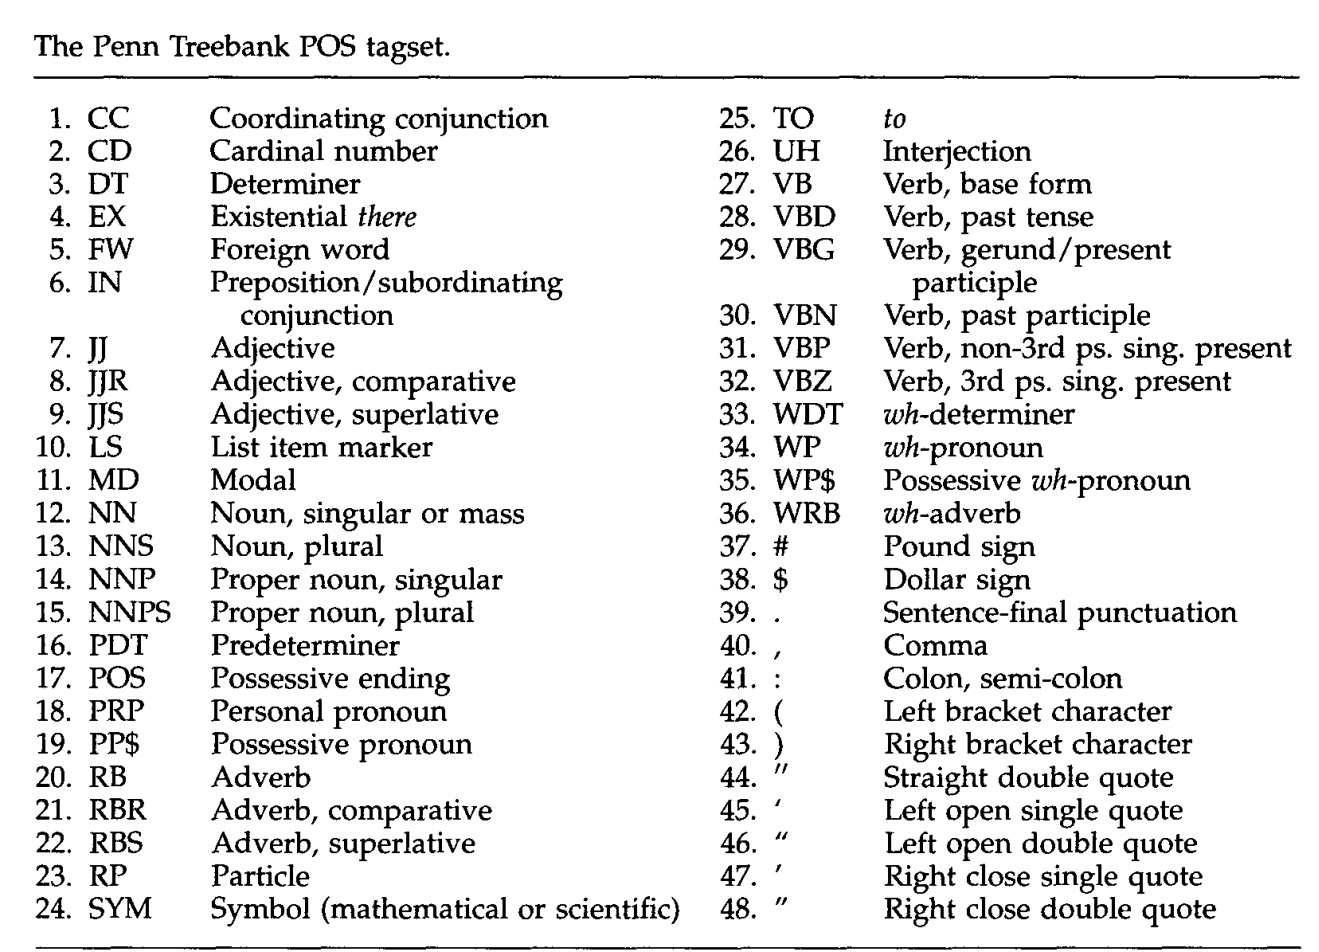
\includegraphics[scale=0.3]{graficos/penn-tagset}
  \caption{Tagset Penn Treebank}
  \label{fig:tagset-penn}
\end{figure}

%\newline

Por su parte, el pos-tagger español de Freeling, por su naturaleza multilingüe, utiliza el tagset propuesto por el grupo EAGLES (\textit{Expert Advisory Group on Language Engineering Standards})\footnote{\url{http://www.ilc.cnr.it/EAGLES96/home.html}}, una organización europea que fomenta la investigación multilingüe, mientras que por una cuestión de compatibilidad, se preservan los tags de Penn Treebank para el inglés. Los tags de EAGLES tienen en consideración diferentes matices para contemplar las variaciones de diferentes idiomas. Sobre un conjunto inicial de 12 categorías -las 9 recién enunciadas más \sq{Signos de puntuación}, \sq{Numerales} y \sq{Fechas y horas} define etiquetas mucho más especificas. En concreto, un tag consta de entre 6 y 7  posiciones, cada una de las cuales expresa una caracteristica de la palabra dependiendo del valor especificado en la posición anterior. Para algunas clases alguno de estos valores no tienen sentido, mientras que para algunas palabras algunos valores no están o no pueden definirse (en el caso de subespecificación de un atributo, esta se nota como un \sq{0}). 
A continuación presentamos la especificación para el conjunto de tags relacionados con sustantivos y un ejemplo de su aplicación.

\begin{center}
\begin{tabular}{| l | l | l | l |}
 \hline
 \multicolumn{4}{|c|}{Nombres} \\ \hline
Pos. & Atributo & Valor & Código \\ \hline
1 & Categoría &  Nombre & N \\ \hline
\multirow{2}{*}{2} & \multirow{2}{*}{Tipo} & Común  & C \\ \cline{3-4}
  & &      Propio & P \\ \hline
\multirow{3}{*}{3} & \multirow{3}{*}{Género} & Masculino & M \\ \cline{3-4}
 & & Femenino &  F \\ \cline{3-4}
 & & Común    & C  \\ \hline
\multirow{3}{*}{4} & \multirow{3}{*}{Número} & Singular & S \\ \cline{3-4}
 & & Plural &  P \\ \cline{3-4}
 & & Invariable & N  \\ \hline
 \multirow{4}{*}{5-6} & \multirow{4}{*}{Clasificación Semántica} & Persona & SP \\ \cline{3-4}
 & & Lugar &  G0 \\ \cline{3-4}
 & & Organización &  O0 \\ \cline{3-4}
 & & Otros & V0  \\ \hline
\multirow{2}{*}{7} & \multirow{2}{*}{Grado} & Aumentativo  & A \\ \cline{3-4}
  & & Disminutivo & D \\ \hline
\end{tabular}
\end{center}


\begin{center}
\begin{tabular}{| l | l | l |}
 \hline
Forma & Lema & Etiqueta \\ \hline 
chico & chico & NCMS000 \\ \hline
chicas & chico & NCFP000 \\ \hline
gatito & gato & NCMS00D \\ \hline
oyente & oyente & NCCS000 \\ \hline
oyentes & oyente & NCCP000 \\ \hline
cortapapeles & cortapapeles &NCMN000 \\ \hline
tesis & tesis & NCFN000 \\ \hline
Barcelona & barcelona & NP000G0 \\ \hline
COI & coi & NP000O0 \\ \hline
Pedro & pedro & NP000P0 \\ \hline
\end{tabular}
\end{center}


Existen varios enfoques algoritmicos al problema del POS tagging: desde los más primitivos basados en reglas escritas a mano pasando a los basados en HMMs (Hidden Markov Models), Maximum Entropy o Transformation Based Learning. Un detalle de estos métodos excede la introducción al problema que supone esta sección de la tesis. El POS tagger de Freeling está basado en el approach de HMMs y el de Stanford en el de Maximum Entropy, ambos modelos de machine learning. En \allref{subsec:freeling-pos} y \allref{sec:stanford-pos} se encuentran algunos comentarios más técnico de los algoritmos de POS tagging que utilizamos en este trabajo y vinculos a bibliografía pertinente y en la sección siguente \allref{subsec:nerc} veremos una descripción más detallada de enfoques algorítmicos al problema que ilustrarán, al menos de modo general, la estructura de la algoritmía basada en machine learning aplicada a procesamiento de lenguajes. 
A continuación listamos ejemplos concretos de análisis de la oración de ejemplo del comienzo de esta sección (\dq{El hombre bajó la escalera.}) para mostrar un funcionamiento real de los algoritmos utilizados en esta tesis. 


\begin{center}
\begin{tabular}{| l | l | l |}
\hline
\multicolumn{3}{|c|}{Freeling (ES)} \\ \hline
Forma &  Etiqueta & Descripción \\ \hline 
El & DA0MS0 & Determinante, Artículo, Másculino, Singular\\ \hline 
hombre & NCMS000 & Nombre, Común, Másculino, Singular  \\ \hline 
bajó & VMIS3S0 & Verbo, Principal, Indicativo, Pasado, Tercera Persona, Singular\\ \hline 
la & DA0FS0 & Determinante, Artículo, Femenino, Singular\\ \hline 
escalera& NCFS000 & Nombre, Común, Femenino, Singular \\ \hline 
.& Fp& Punto final\\ \hline \hline
\multicolumn{3}{|c|}{Freeling (EN)} \\ \hline
Forma & Etiqueta & Descripción \\ \hline 
The &DT & Determiner \\ \hline 
man &NN & Noun, singular or mass \\ \hline 
came  &VBD& Verb, past tense\\ \hline 
down  &RP& Particle \\ \hline 
the &DT& Determiner \\ \hline 
stairs & NNS& Noun, plural \\ \hline 
.& Fp& Sentence final punctuation \\ \hline \hline
\multicolumn{3}{|c|}{Stanford (EN)} \\ \hline
Forma & Etiqueta & Descripción \\ \hline 
The &DT & Determiner \\ \hline 
 man & NN & Noun, singular or mass \\ \hline 
  came &VBD  & Verb, past tense \\ \hline 
 down & RP  &  Particle\\ \hline 
 the & DT  &  Determiner \\ \hline 
 stairs. &NN   & Noun, plural \\ \hline 
 \end{tabular}
\end{center}

En el scope de este proyecto, utilizamos pos-tagging para filtrar clases de palabras inútiles y para seleccionar tres tipos: las qwords, los verbos y los sustantivos (Las qwords son los pronombres interrogativos: qué, quién, cómo, etc. y en inglés, who, when, where...). \newline


\subsection{Named Entity Recognition (NER)}
\label{subsec:nerc}
El reconocimiento de entidades nombradas (NER, de Named Entity
Recognition) es una subtarea de Information Extraction. Information
Extraction es, brevemente, todo el dominio de problemas vinculado con
la extracción de información estructurada a partir de datos no
estructurados o semi estructurados. NER es, dentro de este dominio, el
proceso de reconocer unidades de información (las entidades
nombradas) tales como nombres de personas, organizaciones, lugares,
expresiones numéricas como tiempo, fechas, dinero, porcentajes, etc.
A veces se habla de NERC (Named Entity Recognition and Classification)
para poner énfasis en la asignación de un tipo (por ejemplo: nombre
de empresa) a la entidad nombrada reconocida.

Los primeros sistemas de NER eran algoritmos basados en reglas
hardcodeadas, mientras que los más modernos incorporan técnicas de
machine learning y son, en general, algoritmos basados en features
(ciertos aspectos de los tokens).

El primer sistema data de 1991 y constaba de reglas escritas a mano y
heurísticas simples. Recién en 1996, con el estímulo de la MUC-6
(una conferencia reconocida en el área que dedicó una edición a
NER), el área comenzó a acelerar su crecimiento.

[[En construcción en documento NER de GDrive]]


\subsection{Question Classification}
\label{subsec:qc}
Question Classification es la tarea de categorizar preguntas en diferentes 
clases semánticas que impongan restricciones significativas a las respuestas potenciales 
para utilizarlas en fases posteriores del proceso de QA.
La clasificación de preguntas es una subclase del problema de la clasificación. 
Un clasificador es una herramienta que asigna a un elemento una de
\textit{k} clases. La clasificación es un área bastante fecunda de nlp y, más en general, de machine learning. 
Los clasificadores de preguntas son herramientas que clasifican preguntas según su tipo de respuesta esperada. Por ejemplo:
\dq{?`Quién descubrió América?} espera, más allá del nombre concreto, \textit{un nombre de persona}; {\textquotedblleft}?`Cuándo se descubrió
América?{\textquotedblright} espera \textit{una fecha} (o, más en
general, \textit{un tiempo}), {\textquotedblleft}?`Dónde se
descubrió América?{\textquotedblright} espera, como respuesta,
\textit{un lugar}, etc. Este es un eje de clasificación conocido como
tipo de respuesta esperado, aunque existen otros. Notar que este último ejemplo, en concreto confuso (¿tiene sentido la pregunta?), no lo es a nivel estructural.

El rol del módulo de QC en un sistema de QA es doble: Por un lado, impoen restricciones a la respuesta final, permitiendo filtrar y verificar respuestas candidatas.
Por otra lado, provee información para estructurar el flujo de código de los procesos subsiguientes, permitiendo implementar estrategias puntuales para cada tipo de respuesta esperada. Por ejemplo, para la pregunta \dq{?`Quién fue el primer presidente constitucional de Argentina?} resulta de gran utilidad, a la hora de evaluar pasajes, saber que la respuesta esperada debe ser una \textit{persona}: de este modo se puede evitar el procesamiento lingüístico de un gran dominio de pasajes no relevantes. Estas mismas razones justifican la deseabilidad de la especificidad: saber que la respuesta final debe ser un \textit{presidente} o un \textit{político} es más informativo y útil para el resto del proceso que solo saber que es una \textit{persona}.

Debido a la complejidad de análisis lingüístico intrinseca en la clasificación específica, los sistemas de QC más básicos adoptan un esquema de clases acotado y basado en reglas simples. Típicamente, las clases son: \textit{Persona}, \textit{Lugar}, \textit{Organización}, \textit{Fecha}, \textit{Cantidad}, \textit{Duración}, \textit{Medida}, mientras las reglas de clasificación son parecidas a las siguientes:
\begin{itemize}
\item Si la pregunta empieza con \textit{Quién} o \textit{Quiénes}, entonces el tipo es \textit{Persona}
\item Si la pregunta empieza con \textit{Dónde}, entonces el tipo es \textit{Lugar}
\item Si la pregunta empieza con \textit{Cuándo}, entonces el tipo es \textit{Fecha}
\item Si la pregunta empieza con \textit{Qué}, entonces determinar el tipo de acuerdo al sustantivo principal de la pregunta (utilizando pos-tagging)
\item ...
\end{itemize}

Como nota al pie, este esquema de clasificación semántico es uno entre otros. Por ejemplo, \cite{QC-other} propuso un esquema \textit{conceptual} de 13 clases en las que incluye, por ejemplo: antecedentes y consecuencias causales, habilitación, verificación, disyunción, etc.

Estas reglas básicas -triviales, si se quiere- cubren gran parte de las preguntas con una eficacia alta. En \allref{sec:stanford-qc} veremos un enfoque más complejo que permite una clasificación más granular, basado en machine learning. El uso de algoritmos de machine learning tiene una serie de ventajes interesantes a la hora de definir un sistema de clases complejo. Como mencionamos al hablar de los otros taggers, la definición de reglas manuales es una tarea tediosa y con poca capacidad de adaptarse o modificarse, mientras que la definición de un set de features adecuado para el aprendizaje programático, en cambio, permite la fácil incorporación de nuevas clases y/o la incorporación de nuevas mejoras descubiertas. Por otro lado, un esquema de clases semánticamente rico -más granular que el modelo básico recién enunciado- requiere la consideración de una gran cantidad de dimensiones lingüísticas, tanto sintácticas como semánticas, lo que hace que la definición manual de reglas una tarea potencialmente imposible en terminos de costo de tiempo humano. 

Finalmente, cabe mencionar que no existen clasificadores de preguntas para el español y que a la hora de abordar este problema en nuestra implementación debimos apelar a mecanismos ad-hoc. En particular, para el modelo estructurado implementamos un sistema de reglas simples como el recién enunciado y para el modelo no estructurado utilizamos el resultado de la clasificación de la misma pregunta pero formulada en inglés (pues las preguntas están disponibles en ambos idiomas).
Actualmente, un tesista del grupo GALLI está trabajando en la construcción de un corpus para alimentar un clasificador de preguntas basado en machine learning para el español, pero lamentablemente por cuestiones de tiempos no pudimos hacer uso del mismo en esta tesis.

\section{Otras herramientas}

Esta sección es un placeholder para las siguientes posibles tecnologías que podría describir este capítulo:

\subsection*{Features}
En terminología, una sección explicando features

\subsection*{Coreference Resolution}

Ejemplos de resolución de Freeling.

\subsection*{Word sense disambiguation}

Hablar algo de wordnet ?

\subsection*{Relation Extraction}

La detección y extracción de relaciones es una tarea de procesamiento
de lenguaje natural que consiste en extraer entidades y relaciones semánticas
entre entidades a partir de un texto no estructurado. 

[[Escribir sobre distintos algoritmos conocidos basado en el paper RE1]]

\subsection*{Machine Translation}
Hablar de los problemas con Google y otros y de las memorias de traducción. 

\subsection*{Detección de idiomas}

La detección o identificación de idioma es la tarea de reconocer el
idioma de un cierto contenido. Esta tarea puede pensarse como una
tarea de clasificación donde las clases son los distintos
idiomas que el detector puede reconocer. 

[[Expandir con detalles técnicos de wikipedia]]
